%% bare_jrnl.tex
%% V1.4b
%% 2015/08/26
%% by Michael Shell
%% see http://www.michaelshell.org/
%% for current contact information.
%%
%% This is a skeleton file demonstrating the use of IEEEtran.cls
%% (requires IEEEtran.cls version 1.8b or later) with an IEEE
%% journal paper.
%%
%% Support sites:
%% http://www.michaelshell.org/tex/ieeetran/
%% http://www.ctan.org/pkg/ieeetran
%% and
%% http://www.ieee.org/

%%*************************************************************************
%% Legal Notice:
%% This code is offered as-is without any warranty either expressed or
%% implied; without even the implied warranty of MERCHANTABILITY or
%% FITNESS FOR A PARTICULAR PURPOSE! 
%% User assumes all risk.
%% In no event shall the IEEE or any contributor to this code be liable for
%% any damages or losses, including, but not limited to, incidental,
%% consequential, or any other damages, resulting from the use or misuse
%% of any information contained here.
%%
%% All comments are the opinions of their respective authors and are not
%% necessarily endorsed by the IEEE.
%%
%% This work is distributed under the LaTeX Project Public License (LPPL)
%% ( http://www.latex-project.org/ ) version 1.3, and may be freely used,
%% distributed and modified. A copy of the LPPL, version 1.3, is included
%% in the base LaTeX documentation of all distributions of LaTeX released
%% 2003/12/01 or later.
%% Retain all contribution notices and credits.
%% ** Modified files should be clearly indicated as such, including  **
%% ** renaming them and changing author support contact information. **
%%*************************************************************************


% *** Authors should verify (and, if needed, correct) their LaTeX system  ***
% *** with the testflow diagnostic prior to trusting their LaTeX platform ***
% *** with production work. The IEEE's font choices and paper sizes can   ***
% *** trigger bugs that do not appear when using other class files.       ***                          ***
% The testflow support page is at:
% http://www.michaelshell.org/tex/testflow/



\documentclass[journal]{IEEEtran}
%
% If IEEEtran.cls has not been installed into the LaTeX system files,
% manually specify the path to it like:
% \documentclass[journal]{../sty/IEEEtran}

\usepackage[pdftex]{graphicx}
\graphicspath{{../pdf/}{../jpeg/}}
\DeclareGraphicsExtensions{.pdf,.jpeg,.png}




% Some very useful LaTeX packages include:
% (uncomment the ones you want to load)


% *** MISC UTILITY PACKAGES ***
%
%\usepackage{ifpdf}
% Heiko Oberdiek's ifpdf.sty is very useful if you need conditional
% compilation based on whether the output is pdf or dvi.
% usage:
% \ifpdf
%   % pdf code
% \else
%   % dvi code
% \fi
% The latest version of ifpdf.sty can be obtained from:
% http://www.ctan.org/pkg/ifpdf
% Also, note that IEEEtran.cls V1.7 and later provides a builtin
% \ifCLASSINFOpdf conditional that works the same way.
% When switching from latex to pdflatex and vice-versa, the compiler may
% have to be run twice to clear warning/error messages.






% *** CITATION PACKAGES ***
%
%\usepackage{cite}
% cite.sty was written by Donald Arseneau
% V1.6 and later of IEEEtran pre-defines the format of the cite.sty package
% \cite{} output to follow that of the IEEE. Loading the cite package will
% result in citation numbers being automatically sorted and properly
% "compressed/ranged". e.g., [1], [9], [2], [7], [5], [6] without using
% cite.sty will become [1], [2], [5]--[7], [9] using cite.sty. cite.sty's
% \cite will automatically add leading space, if needed. Use cite.sty's
% noadjust option (cite.sty V3.8 and later) if you want to turn this off
% such as if a citation ever needs to be enclosed in parenthesis.
% cite.sty is already installed on most LaTeX systems. Be sure and use
% version 5.0 (2009-03-20) and later if using hyperref.sty.
% The latest version can be obtained at:
% http://www.ctan.org/pkg/cite
% The documentation is contained in the cite.sty file itself.






% *** GRAPHICS RELATED PACKAGES ***
%
\ifCLASSINFOpdf
  % \usepackage[pdftex]{graphicx}
  % declare the path(s) where your graphic files are
  % \graphicspath{{../pdf/}{../jpeg/}}
  % and their extensions so you won't have to specify these with
  % every instance of \includegraphics
  % \DeclareGraphicsExtensions{.pdf,.jpeg,.png}
\else
  % or other class option (dvipsone, dvipdf, if not using dvips). graphicx
  % will default to the driver specified in the system graphics.cfg if no
  % driver is specified.
  % \usepackage[dvips]{graphicx}
  % declare the path(s) where your graphic files are
  % \graphicspath{{../eps/}}
  % and their extensions so you won't have to specify these with
  % every instance of \includegraphics
  % \DeclareGraphicsExtensions{.eps}
\fi
% graphicx was written by David Carlisle and Sebastian Rahtz. It is
% required if you want graphics, photos, etc. graphicx.sty is already
% installed on most LaTeX systems. The latest version and documentation
% can be obtained at: 
% http://www.ctan.org/pkg/graphicx
% Another good source of documentation is "Using Imported Graphics in
% LaTeX2e" by Keith Reckdahl which can be found at:
% http://www.ctan.org/pkg/epslatex
%
% latex, and pdflatex in dvi mode, support graphics in encapsulated
% postscript (.eps) format. pdflatex in pdf mode supports graphics
% in .pdf, .jpeg, .png and .mps (metapost) formats. Users should ensure
% that all non-photo figures use a vector format (.eps, .pdf, .mps) and
% not a bitmapped formats (.jpeg, .png). The IEEE frowns on bitmapped formats
% which can result in "jaggedy"/blurry rendering of lines and letters as
% well as large increases in file sizes.
%
% You can find documentation about the pdfTeX application at:
% http://www.tug.org/applications/pdftex





% *** MATH PACKAGES ***
%
%\usepackage{amsmath}
% A popular package from the American Mathematical Society that provides
% many useful and powerful commands for dealing with mathematics.
%
% Note that the amsmath package sets \interdisplaylinepenalty to 10000
% thus preventing page breaks from occurring within multiline equations. Use:
%\interdisplaylinepenalty=2500
% after loading amsmath to restore such page breaks as IEEEtran.cls normally
% does. amsmath.sty is already installed on most LaTeX systems. The latest
% version and documentation can be obtained at:
% http://www.ctan.org/pkg/amsmath





% *** SPECIALIZED LIST PACKAGES ***
%
%\usepackage{algorithmic}
% algorithmic.sty was written by Peter Williams and Rogerio Brito.
% This package provides an algorithmic environment fo describing algorithms.
% You can use the algorithmic environment in-text or within a figure
% environment to provide for a floating algorithm. Do NOT use the algorithm
% floating environment provided by algorithm.sty (by the same authors) or
% algorithm2e.sty (by Christophe Fiorio) as the IEEE does not use dedicated
% algorithm float types and packages that provide these will not provide
% correct IEEE style captions. The latest version and documentation of
% algorithmic.sty can be obtained at:
% http://www.ctan.org/pkg/algorithms
% Also of interest may be the (relatively newer and more customizable)
% algorithmicx.sty package by Szasz Janos:
% http://www.ctan.org/pkg/algorithmicx




% *** ALIGNMENT PACKAGES ***
%
%\usepackage{array}
% Frank Mittelbach's and David Carlisle's array.sty patches and improves
% the standard LaTeX2e array and tabular environments to provide better
% appearance and additional user controls. As the default LaTeX2e table
% generation code is lacking to the point of almost being broken with
% respect to the quality of the end results, all users are strongly
% advised to use an enhanced (at the very least that provided by array.sty)
% set of table tools. array.sty is already installed on most systems. The
% latest version and documentation can be obtained at:
% http://www.ctan.org/pkg/array


% IEEEtran contains the IEEEeqnarray family of commands that can be used to
% generate multiline equations as well as matrices, tables, etc., of high
% quality.




% *** SUBFIGURE PACKAGES ***
%\ifCLASSOPTIONcompsoc
%  \usepackage[caption=false,font=normalsize,labelfont=sf,textfont=sf]{subfig}
%\else
%  \usepackage[caption=false,font=footnotesize]{subfig}
%\fi
% subfig.sty, written by Steven Douglas Cochran, is the modern replacement
% for subfigure.sty, the latter of which is no longer maintained and is
% incompatible with some LaTeX packages including fixltx2e. However,
% subfig.sty requires and automatically loads Axel Sommerfeldt's caption.sty
% which will override IEEEtran.cls' handling of captions and this will result
% in non-IEEE style figure/table captions. To prevent this problem, be sure
% and invoke subfig.sty's "caption=false" package option (available since
% subfig.sty version 1.3, 2005/06/28) as this is will preserve IEEEtran.cls
% handling of captions.
% Note that the Computer Society format requires a larger sans serif font
% than the serif footnote size font used in traditional IEEE formatting
% and thus the need to invoke different subfig.sty package options depending
% on whether compsoc mode has been enabled.
%
% The latest version and documentation of subfig.sty can be obtained at:
% http://www.ctan.org/pkg/subfig




% *** FLOAT PACKAGES ***
%
%\usepackage{fixltx2e}
% fixltx2e, the successor to the earlier fix2col.sty, was written by
% Frank Mittelbach and David Carlisle. This package corrects a few problems
% in the LaTeX2e kernel, the most notable of which is that in current
% LaTeX2e releases, the ordering of single and double column floats is not
% guaranteed to be preserved. Thus, an unpatched LaTeX2e can allow a
% single column figure to be placed prior to an earlier double column
% figure.
% Be aware that LaTeX2e kernels dated 2015 and later have fixltx2e.sty's
% corrections already built into the system in which case a warning will
% be issued if an attempt is made to load fixltx2e.sty as it is no longer
% needed.
% The latest version and documentation can be found at:
% http://www.ctan.org/pkg/fixltx2e


%\usepackage{stfloats}
% stfloats.sty was written by Sigitas Tolusis. This package gives LaTeX2e
% the ability to do double column floats at the bottom of the page as well
% as the top. (e.g., "\begin{figure*}[!b]" is not normally possible in
% LaTeX2e). It also provides a command:
%\fnbelowfloat
% to enable the placement of footnotes below bottom floats (the standard
% LaTeX2e kernel puts them above bottom floats). This is an invasive package
% which rewrites many portions of the LaTeX2e float routines. It may not work
% with other packages that modify the LaTeX2e float routines. The latest
% version and documentation can be obtained at:
% http://www.ctan.org/pkg/stfloats
% Do not use the stfloats baselinefloat ability as the IEEE does not allow
% \baselineskip to stretch. Authors submitting work to the IEEE should note
% that the IEEE rarely uses double column equations and that authors should try
% to avoid such use. Do not be tempted to use the cuted.sty or midfloat.sty
% packages (also by Sigitas Tolusis) as the IEEE does not format its papers in
% such ways.
% Do not attempt to use stfloats with fixltx2e as they are incompatible.
% Instead, use Morten Hogholm'a dblfloatfix which combines the features
% of both fixltx2e and stfloats:
%
% \usepackage{dblfloatfix}
% The latest version can be found at:
% http://www.ctan.org/pkg/dblfloatfix




%\ifCLASSOPTIONcaptionsoff
%  \usepackage[nomarkers]{endfloat}
% \let\MYoriglatexcaption\caption
% \renewcommand{\caption}[2][\relax]{\MYoriglatexcaption[#2]{#2}}
%\fi
% endfloat.sty was written by James Darrell McCauley, Jeff Goldberg and 
% Axel Sommerfeldt. This package may be useful when used in conjunction with 
% IEEEtran.cls'  captionsoff option. Some IEEE journals/societies require that
% submissions have lists of figures/tables at the end of the paper and that
% figures/tables without any captions are placed on a page by themselves at
% the end of the document. If needed, the draftcls IEEEtran class option or
% \CLASSINPUTbaselinestretch interface can be used to increase the line
% spacing as well. Be sure and use the nomarkers option of endfloat to
% prevent endfloat from "marking" where the figures would have been placed
% in the text. The two hack lines of code above are a slight modification of
% that suggested by in the endfloat docs (section 8.4.1) to ensure that
% the full captions always appear in the list of figures/tables - even if
% the user used the short optional argument of \caption[]{}.
% IEEE papers do not typically make use of \caption[]'s optional argument,
% so this should not be an issue. A similar trick can be used to disable
% captions of packages such as subfig.sty that lack options to turn off
% the subcaptions:
% For subfig.sty:
% \let\MYorigsubfloat\subfloat
% \renewcommand{\subfloat}[2][\relax]{\MYorigsubfloat[]{#2}}
% However, the above trick will not work if both optional arguments of
% the \subfloat command are used. Furthermore, there needs to be a
% description of each subfigure *somewhere* and endfloat does not add
% subfigure captions to its list of figures. Thus, the best approach is to
% avoid the use of subfigure captions (many IEEE journals avoid them anyway)
% and instead reference/explain all the subfigures within the main caption.
% The latest version of endfloat.sty and its documentation can obtained at:
% http://www.ctan.org/pkg/endfloat
%
% The IEEEtran \ifCLASSOPTIONcaptionsoff conditional can also be used
% later in the document, say, to conditionally put the References on a 
% page by themselves.




% *** PDF, URL AND HYPERLINK PACKAGES ***
%
%\usepackage{url}
% url.sty was written by Donald Arseneau. It provides better support for
% handling and breaking URLs. url.sty is already installed on most LaTeX
% systems. The latest version and documentation can be obtained at:
% http://www.ctan.org/pkg/url
% Basically, \url{my_url_here}.




% *** Do not adjust lengths that control margins, column widths, etc. ***
% *** Do not use packages that alter fonts (such as pslatex).         ***
% There should be no need to do such things with IEEEtran.cls V1.6 and later.
% (Unless specifically asked to do so by the journal or conference you plan
% to submit to, of course. )


% correct bad hyphenation here
\hyphenation{op-tical net-works semi-conduc-tor}


\begin{document}
\bstctlcite{IEEEexample:BSTcontrol}
%
% paper title
% Titles are generally capitalized except for words such as a, an, and, as,
% at, but, by, for, in, nor, of, on, or, the, to and up, which are usually
% not capitalized unless they are the first or last word of the title.
% Linebreaks \\ can be used within to get better formatting as desired.
% Do not put math or special symbols in the title.
\title{Augmented Reality by Hand Gesture Recognized Commands and Movements}
%
%
% author names and IEEE memberships
% note positions of commas and nonbreaking spaces ( ~ ) LaTeX will not break
% a structure at a ~ so this keeps an author's name from being broken across
% two lines.
% use \thanks{} to gain access to the first footnote area
% a separate \thanks must be used for each paragraph as LaTeX2e's \thanks
% was not built to handle multiple paragraphs
%

\author{MEHDI VALINEJAD,~\IEEEmembership{Student}.
MOHAMMADYOUSEF SADRIALAMDARI,~\IEEEmembership{Student}% <-this % stops a space
% \thanks{M. Shell was with the Department
% of Electrical and Computer Engineering, Georgia Institute of Technology, Atlanta,
% GA, 30332 USA e-mail: (see http://www.michaelshell.org/contact.html).}% <-this % stops a space
% \thanks{J. Doe and J. Doe are with Anonymous University.}% <-this % stops a space
% \thanks{Manuscript received April 19, 2005; revised August 26, 2015.}
}

% note the % following the last \IEEEmembership and also \thanks - 
% these prevent an unwanted space from occurring between the last author name
% and the end of the author line. i.e., if you had this:
% 
% \author{....lastname \thanks{...} \thanks{...} }
%                     ^------------^------------^----Do not want these spaces!
%
% a space would be appended to the last name and could cause every name on that
% line to be shifted left slightly. This is one of those "LaTeX things". For
% instance, "\textbf{A} \textbf{B}" will typeset as "A B" not "AB". To get
% "AB" then you have to do: "\textbf{A}\textbf{B}"
% \thanks is no different in this regard, so shield the last } of each \thanks
% that ends a line with a % and do not let a space in before the next \thanks.
% Spaces after \IEEEmembership other than the last one are OK (and needed) as
% you are supposed to have spaces between the names. For what it is worth,
% this is a minor point as most people would not even notice if the said evil
% space somehow managed to creep in.



% The paper headers
\markboth{Augmented Reality by Hand Gesture Recognized Commands and Movements, VOL.~01, NO.~01, DECEMBER~2023}%
{Shell \MakeLowercase{\textit{et al.}}: Augmented Reality by Hand Gesture Recognized Commands and Movements}
% The only time the second header will appear is for the odd numbered pages
% after the title page when using the twoside option.
% 
% *** Note that you probably will NOT want to include the author's ***
% *** name in the headers of peer review papers.                   ***
% You can use \ifCLASSOPTIONpeerreview for conditional compilation here if
% you desire.




% If you want to put a publisher's ID mark on the page you can do it like
% this:
%\IEEEpubid{0000--0000/00\$00.00~\copyright~2015 IEEE}
% Remember, if you use this you must call \IEEEpubidadjcol in the second
% column for its text to clear the IEEEpubid mark.



% use for special paper notices
%\IEEEspecialpapernotice{(Invited Paper)}




% make the title area
\maketitle

% As a general rule, do not put math, special symbols or citations
% in the abstract or keywords.
\begin{abstract}
The abstract goes here.
\end{abstract}

% Note that keywords are not normally used for peerreview papers.
\begin{IEEEkeywords}
Computer Vision, HCI, Hand Gesture Recognition, Augmented Reality, ArUaco Markers, Landmark, MediaPipe.
\end{IEEEkeywords}






% For peer review papers, you can put extra information on the cover
% page as needed:
% \ifCLASSOPTIONpeerreview
% \begin{center} \bfseries EDICS Category: 3-BBND \end{center}
% \fi
%
% For peerreview papers, this IEEEtran command inserts a page break and
% creates the second title. It will be ignored for other modes.
\IEEEpeerreviewmaketitle



% The very first letter is a 2 line initial drop letter followed
% by the rest of the first word in caps.
% 
% form to use if the first word consists of a single letter:
% \IEEEPARstart{A}{demo} file is ....
% 
% form to use if you need the single drop letter followed by
% normal text (unknown if ever used by the IEEE):
% \IEEEPARstart{A}{}demo file is ....
% 
% Some journals put the first two words in caps:
% \IEEEPARstart{T}{his demo} file is ....
% 
% Here we have the typical use of a "T" for an initial drop letter
% and "HIS" in caps to complete the first word.
\section{Introduction}

\IEEEPARstart{T}{he} Human-Computer Interaction (HCI) represents a nuanced and interdisciplinary domain that intricately 
investigates the symbiotic relationship between humans and computer systems, with a primary focus on optimizing the design 
and utilization of technological interfaces. At its core, HCI delves into the intricacies of how individuals interact with 
computing devices, aiming to refine and elevate these interactions to levels of heightened effectiveness, efficiency, and 
overall user satisfaction.


Hand gesture recognition plays a significant role in Human-Computer Interaction (HCI) by providing a natural and intuitive means 
for users to interact with computers and devices. The relationship between hand gesture recognition and HCI lies in the application 
of gesture-based interfaces to enhance the way users communicate with and control technology. 

Augmented Reality (AR) is a technology that overlays digital information and virtual objects on the real-world environment, 
creating an augmented view for users. Unlike virtual reality, which immerses users in a completely computer-generated environment, 
augmented reality enhances the real-world environment by adding computer-generated perceptual information.

The relationship between Human-Computer Interaction (HCI) and Augmented Reality (AR) is profound, as AR technologies heavily 
rely on effective HCI principles to deliver immersive and user-friendly experiences. Some of their interconnection aspects can 
be noted as User Interface and User Experience Design, Motion and Gesture Interaction, Spatial Awareness, Usability in 3D space, 
Feedback and user guidance, Context-Aware Computing, Accessibility in AR.

In recent years, the integration of cutting-edge technologies has propelled Human-Computer Interaction (HCI) to new heights, 
revolutionizing the way users engage with digital content. One captivating synergy within this realm lies at the intersection 
of Hand Gesture Recognition (HGR) and Marker-Based Augmented Reality (AR). This amalgamation presents a promising frontier for 
creating intuitive and immersive interactive experiences, where users can seamlessly navigate and manipulate augmented environments 
through natural hand gestures.

Hand gesture recognition, a pivotal facet of HCI, enables users to communicate with computing systems using natural and instinctive 
movements. Leveraging advanced computer vision algorithms, these systems interpret and respond to the intricacies of hand gestures, 
introducing an unparalleled level of intuitiveness to human-computer interactions. Concurrently, Marker-Based Augmented Reality 
employs identifiable markers, such as QR codes or images, as triggers to overlay digital content onto the physical world. 
This technology augments reality by blending virtual elements with the user's immediate environment.

The convergence of hand gesture recognition and marker-based AR holds great promise for advancing the field of HCI. By integrating 
gesture recognition into AR interfaces, users can interact with digital content in a manner that mirrors real-world actions, 
fostering a more intuitive and engaging experience. This marriage of technologies addresses the limitations of traditional input methods, 
offering a more natural, efficient, and hands-free mode of interaction within augmented environments.

This paper explores the synergy between hand gesture recognition and marker-based AR, examining the implications for user interface 
design, interactive applications, and the overall user experience. We delve into the technical intricacies of combining these 
technologies, exploring how gesture-driven interactions can enhance the usability and accessibility of marker-based AR systems. 
Moreover, we investigate the potential impact on diverse application domains, from gaming and education to industrial training and 
collaborative workspaces.

As we navigate through the intricate landscape of this technological convergence, we seek to unravel the synergies and challenges 
that arise when marrying hand gesture recognition with marker-based AR. By doing so, we aim to contribute to the ongoing discourse 
in HCI, providing insights that inform the design and development of more natural and immersive interfaces for augmented reality environments. 
The journey into this fusion promises to unlock novel possibilities, shaping the future landscape of interactive technologies and user experiences.










% === II. Planned Methods ========================
% =================================================================================
\section{Planned Methods and Tools}


\subsection*{1. Landmark Detection}
Landmark detection, also known as keypoint detection, refers to the process of identifying and locating specific points or 
features within an image or a visual scene. These points are often distinctive and can be used as references or landmarks 
for various computer vision tasks. Landmark detection is a crucial step in understanding and analyzing images, enabling applications 
in fields such as facial recognition, pose estimation, object tracking, and augmented reality \cite{lin2021ego2hands}.

MediaPipe utilizes a specific model called the MediaPipe Hands for hand tracking, including hand landmark detection. 
The algorithm for hand landmark detection in MediaPipe Hands is based on a convolutional neural network (CNN) architecture.

The hand landmark model in MediaPipe can detect and track 21 3D landmarks on each hand, including key points such as the tips 
of the fingers, the base of the palm, and points along the hand contours. This enables precise tracking and recognition of hand 
gestures in real-time video or image streams.

\begin{figure}[!t]
  \centering
  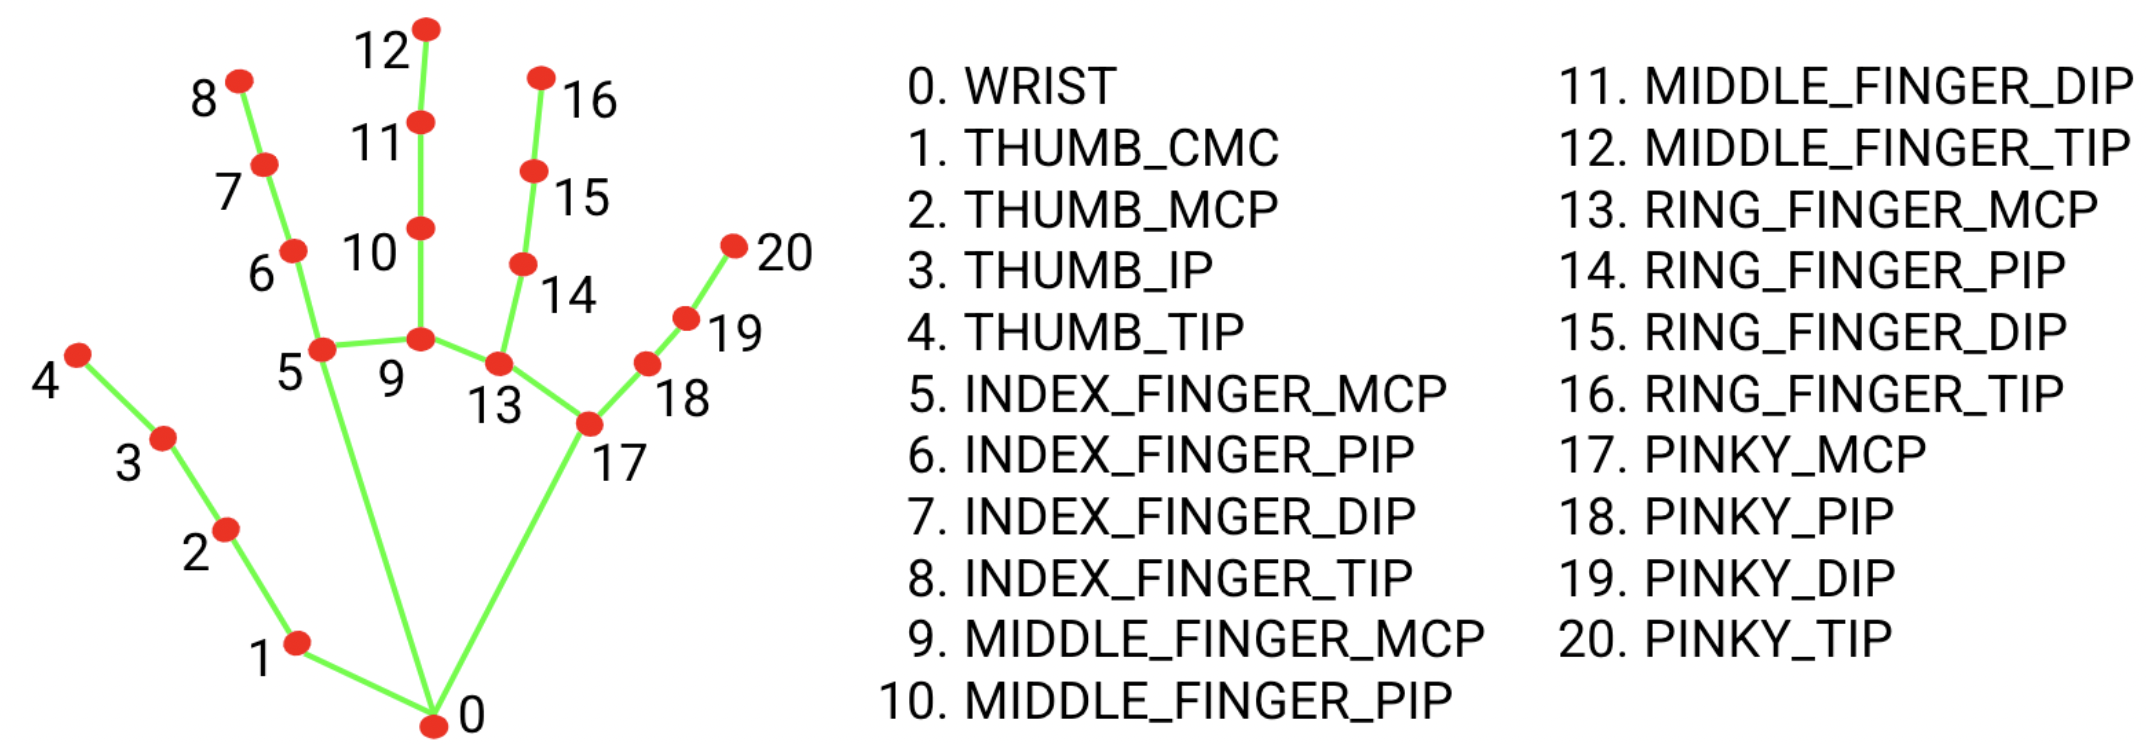
\includegraphics[width=3.5in]{photo/hand-landmarks.png}
  The list of detected point of the hand by landmark hand detector.
  \caption{Landmark hand gesture detected joints}
  \label{fig_sim}
\end{figure}

\subsection*{2. ArUco markers}

ArUco markers are a type of augmented reality marker designed for computer vision applications, particularly for tasks such as 
camera calibration and augmented reality (AR) systems. These markers are black-and-white square patterns that are easy to detect 
and identify in images or video frames. using markers we are able to detect critical points in an video stream frame, generally, 
markers are used for Visual Pattern Recognition, Unique identification, camera calibration and etc. 

OpenCV (Open Source Computer Vision Library) provides a dedicated module for ArUco marker detection, and the implementation is 
based on the ArUco library. The ArUco module in OpenCV is specifically designed for easy integration of ArUco markers into 
computer vision applications.

\subsection*{3. Homography Finding}

To estimate the transformation matrix (homography matrix) that relates corresponding points in two images of the same scene. OpenCV
offers builtin homography detection methods that can be used for perspective point matching between real image and the way of residing 
in the the parent image visible area.

\begin{figure}[!t]
  \centering
  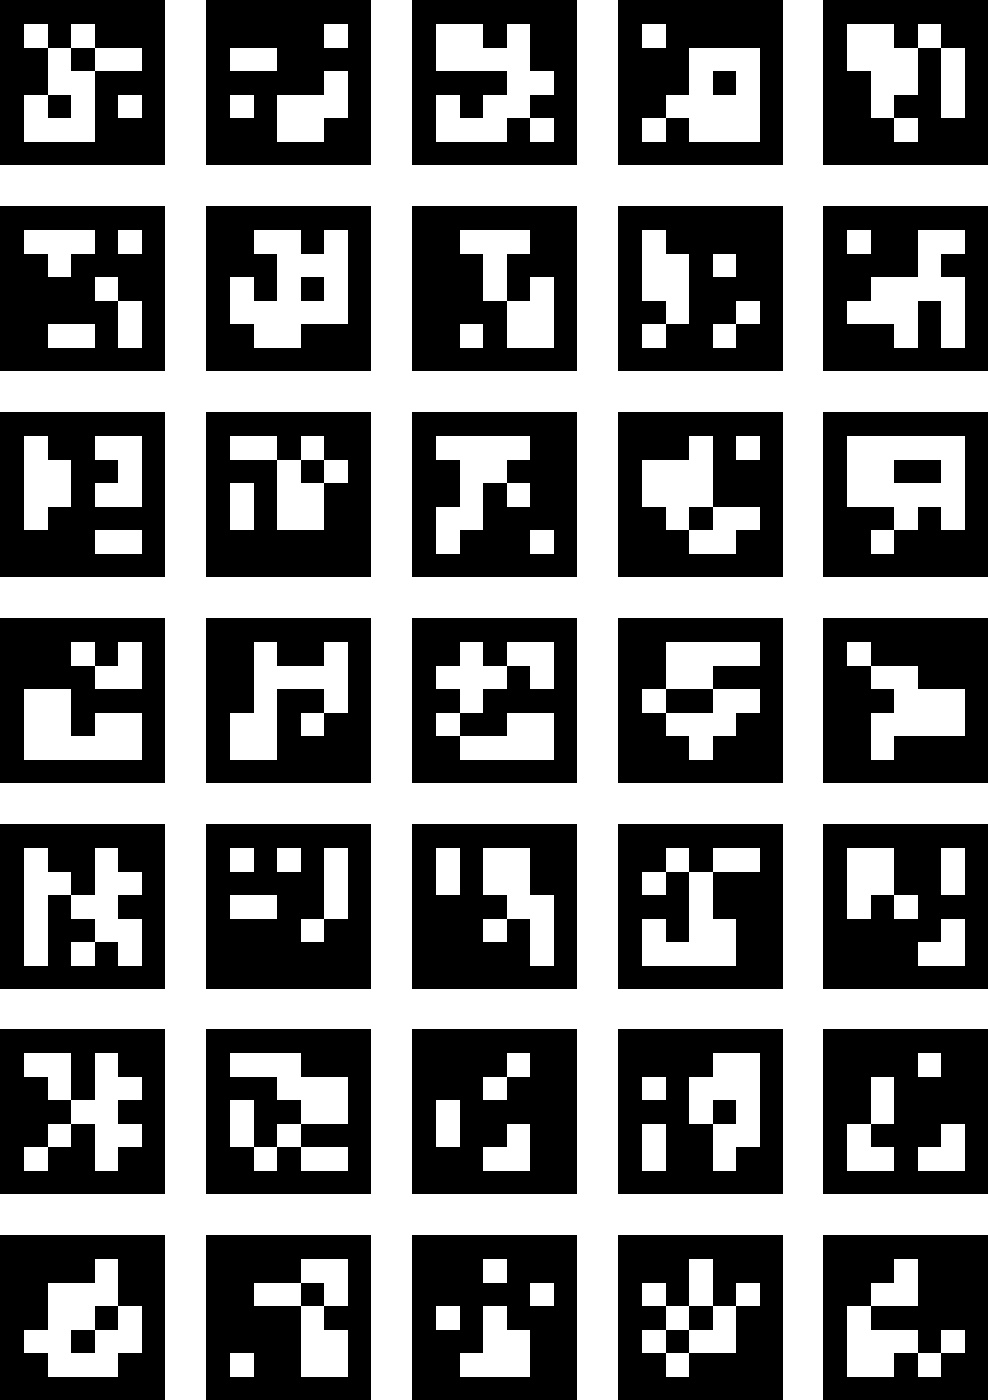
\includegraphics[width=1.5in]{photo/aruco-markers.png}
  Sample chart of ArUco Markers.
  \caption{ArUco Markers}
  \label{fig_sim}
\end{figure}

\section{Expected Results}

The expected result of landmark-based hand gesture detection combined with augmented reality (AR) can be a dynamic and interactive 
user experience where real-world hand movements are used to control and interact with virtual elements. 
Here's an overview of the potential outcomes:
\subsection*{Real-Time Hand Gesture Detection}
Accurate and real-time detection of hand gestures using landmarks provides a natural and intuitive way for users to convey commands or 
interact with digital content.
\subsection*{Precise Tracking of Hand Poses}
Landmark detection allows for precise tracking of the positions and orientations of key points on the hand, enabling accurate 
recognition of various hand poses and movements.
\subsection*{Virtual Object Manipulation}
Users can interact with virtual objects overlaid on the real-world environment using their hand gestures. This could include 
grabbing, moving, rotating, or resizing virtual elements.
\subsection*{Gesture-Based Controls}
Hand gestures can serve as a gesture-based control interface for AR applications. For example, a specific gesture might trigger 
an event, change the color or view, or initiate a specific action.
\subsection*{Immersive AR Experiences}
Landmark-based hand gesture detection enhances the immersion of AR experiences by allowing users to engage with the virtual 
content in a more natural and hands-on manner.
\subsection*{Natural Interaction in AR Painting}
In AR painting game, users can control characters or perform in-game actions using hand gestures detected by landmarks. This adds a 
layer of physicality and engagement to the painting experience.
\subsection*{Overall Expectation}
The expected result is an interactive and immersive AR experience where users can use their hands and gestures to 
manipulate digital content, enhancing the naturalness and engagement of human-computer interactions in augmented reality.




% An example of a floating figure using the graphicx package.
% Note that \label must occur AFTER (or within) \caption.
% For figures, \caption should occur after the \includegraphics.
% Note that IEEEtran v1.7 and later has special internal code that
% is designed to preserve the operation of \label within \caption
% even when the captionsoff option is in effect. However, because
% of issues like this, it may be the safest practice to put all your
% \label just after \caption rather than within \caption{}.
%
% Reminder: the "draftcls" or "draftclsnofoot", not "draft", class
% option should be used if it is desired that the figures are to be
% displayed while in draft mode.
%
% \begin{figure}[!t]
% \centering
% 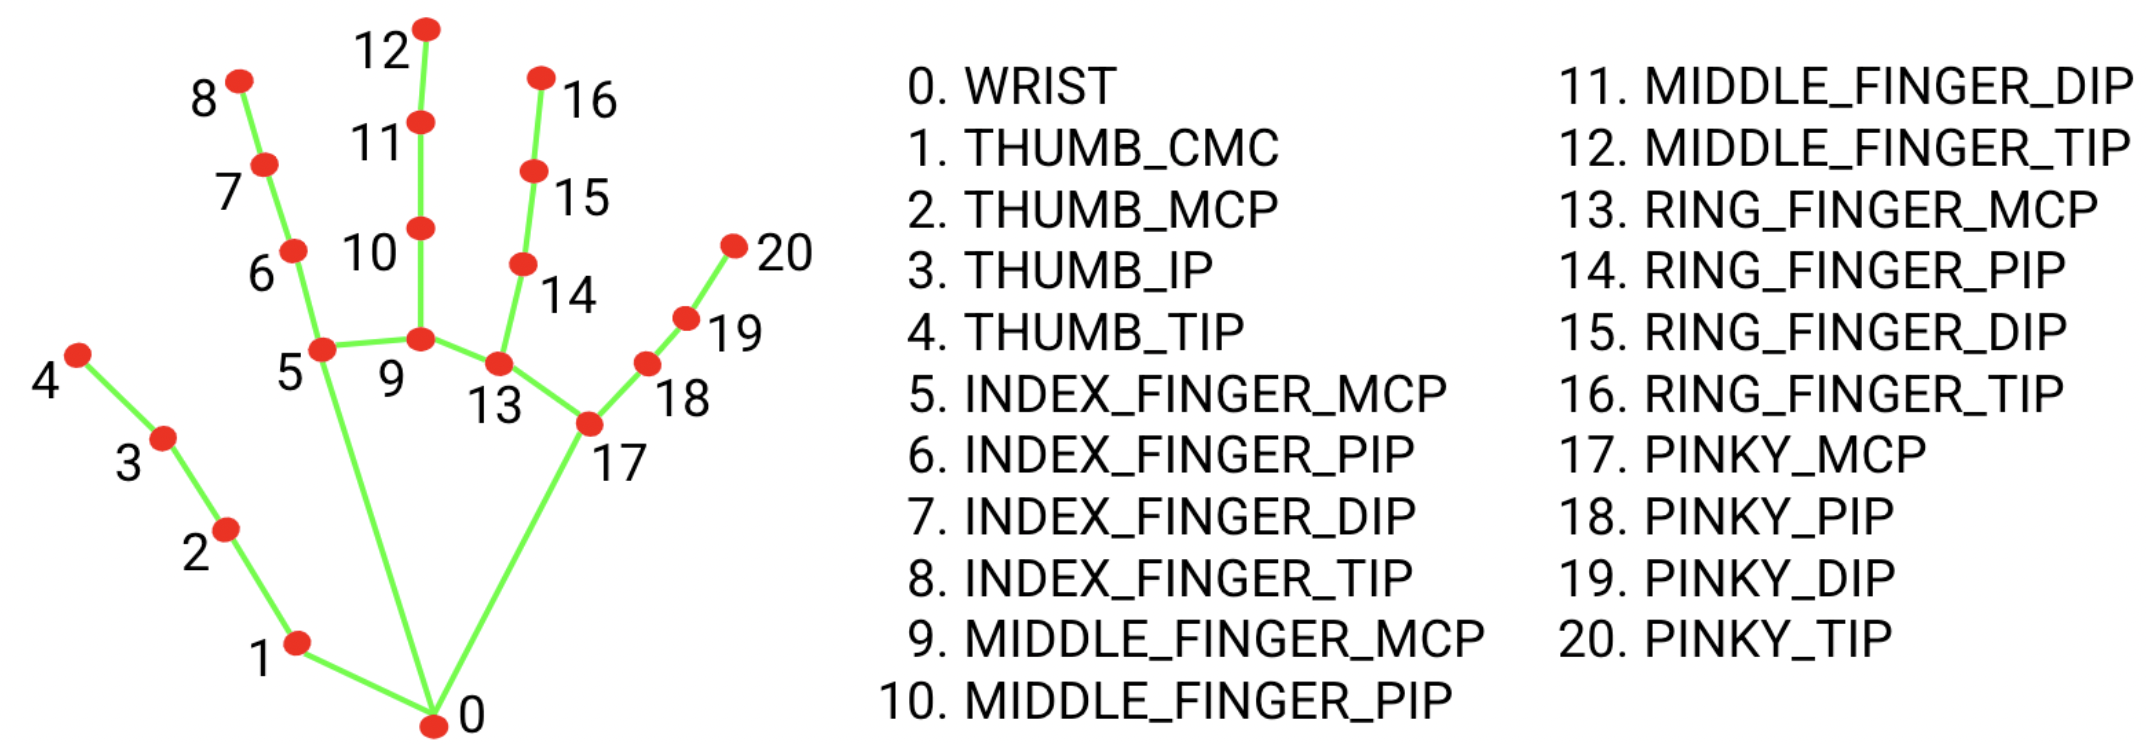
\includegraphics[width=3.5in]{photo/hand-landmarks.png}
% where an .eps filename suffix will be assumed under latex, 
% and a .pdf suffix will be assumed for pdflatex; or what has been declared
% via \DeclareGraphicsExtensions.
% \caption{Simulation results for the network.}
% \label{fig_sim}
% \end{figure}

% Note that the IEEE typically puts floats only at the top, even when this
% results in a large percentage of a column being occupied by floats.


% An example of a double column floating figure using two subfigures.
% (The subfig.sty package must be loaded for this to work.)
% The subfigure \label commands are set within each subfloat command,
% and the \label for the overall figure must come after \caption.
% \hfil is used as a separator to get equal spacing.
% Watch out that the combined width of all the subfigures on a 
% line do not exceed the text width or a line break will occur.
%
%\begin{figure*}[!t]
%\centering
%\subfloat[Case I]{\includegraphics[width=2.5in]{box}%
%\label{fig_first_case}}
%\hfil
%\subfloat[Case II]{\includegraphics[width=2.5in]{box}%
%\label{fig_second_case}}
%\caption{Simulation results for the network.}
%\label{fig_sim}
%\end{figure*}
%
% Note that often IEEE papers with subfigures do not employ subfigure
% captions (using the optional argument to \subfloat[]), but instead will
% reference/describe all of them (a), (b), etc., within the main caption.
% Be aware that for subfig.sty to generate the (a), (b), etc., subfigure
% labels, the optional argument to \subfloat must be present. If a
% subcaption is not desired, just leave its contents blank,
% e.g., \subfloat[].


% An example of a floating table. Note that, for IEEE style tables, the
% \caption command should come BEFORE the table and, given that table
% captions serve much like titles, are usually capitalized except for words
% such as a, an, and, as, at, but, by, for, in, nor, of, on, or, the, to
% and up, which are usually not capitalized unless they are the first or
% last word of the caption. Table text will default to \footnotesize as
% the IEEE normally uses this smaller font for tables.
% The \label must come after \caption as always.
%
%\begin{table}[!t]
%% increase table row spacing, adjust to taste
%\renewcommand{\arraystretch}{1.3}
% if using array.sty, it might be a good idea to tweak the value of
% \extrarowheight as needed to properly center the text within the cells
%\caption{An Example of a Table}
%\label{table_example}
%\centering
%% Some packages, such as MDW tools, offer better commands for making tables
%% than the plain LaTeX2e tabular which is used here.
%\begin{tabular}{|c||c|}
%\hline
%One & Two\\
%\hline
%Three & Four\\
%\hline
%\end{tabular}
%\end{table}


% Note that the IEEE does not put floats in the very first column
% - or typically anywhere on the first page for that matter. Also,
% in-text middle ("here") positioning is typically not used, but it
% is allowed and encouraged for Computer Society conferences (but
% not Computer Society journals). Most IEEE journals/conferences use
% top floats exclusively. 
% Note that, LaTeX2e, unlike IEEE journals/conferences, places
% footnotes above bottom floats. This can be corrected via the
% \fnbelowfloat command of the stfloats package.


\section{Implemented Method}
\subsection*{Gesture Detection}
The formalized design and development of a Python-based application represent a conscientious endeavor to harness real-time webcam 
video streams and exploit the functionalities of the MediaPipe library, incorporating a landmark hand gesture detection model. 
The objective of this application is to solicit user commands through discerning Victory and Thumb Up hand gestures. The framework 
further accommodates the tracking of the index finger tip's spatial coordinates on the screen, leveraging these movements to 
effectuate a drawing mechanism, metaphorically akin to the operation of a pen with the index finger tip serving as the point of contact.

This application establishes a robust command-handling mechanism within the detector module, facilitating the interpretation of user
 gestures and triggering specific actions accordingly. In particular, the application is configured to capture the screen, inclusive 
 of the ongoing drawing, upon the issuance of a specific command.

The intricacies of the application's design are rooted in its capacity to engage with the webcam's live video feed, an attribute that 
epitomizes real-time interaction. The utilization of the MediaPipe library augments this capability by seamlessly integrating landmark 
detection models, offering precise tracking of salient points on the user's hand, particularly focusing on the Victory and Thumb Up gestures.

Moreover, the nuanced tracking of the index finger tip emerges as a pivotal feature, enabling users to articulate their creative 
expressions by translating the finger's movements into a dynamic drawing interface. The application’s gesture recognition module is 
adept at discerning predefined hand poses, such as Victory and Thumb Up, transforming them into actionable commands within the 
application's framework.

The comprehensive command-handling module is instrumental in orchestrating specific responses to detected gestures. In this context, 
the capability to capture screenshots encapsulating the current screen, inclusive of any ongoing drawings, underscores the versatility
 of this application as a tool for creative expression and documentation.

This formalized application, blending Python programming language with advanced computer vision techniques, exemplifies a paradigm 
shift in the realm of interactive systems. It not only underscores the convergence of webcam video stream analysis and landmark hand 
gesture detection but also signifies a synthesis of practical utility and creative expression. As technology continues to evolve, 
this formalized approach provides a testament to the adaptability and innovation inherent in applications that harmoniously integrate 
real-time video analysis and human-computer interaction.

\subsection*{Augmented reality}
Augmenting the aforementioned application's capabilities, the incorporation of ArUco markers introduces an augmented reality (AR) 
dimension to the framework. This strategic integration enriches the user experience by seamlessly aligning the screenshots, captured 
through hand gesture commands, within the context of discernible ArUco markers. The symbiosis of these markers and the application's 
responsive mechanisms supports dynamic movement and perspective transformations, facilitated by rigorous homography calculations.

The introduction of ArUco markers serves as a pivotal element in bridging the virtual and physical realms within the AR paradigm. 
These markers, strategically placed within the physical environment, become reference points that anchor the AR content. 
The screenshots obtained through hand gesture commands seamlessly inhabit this augmented space, aligning with the markers and adapting 
to changes in movement and perspective.

The application, thus, leverages homography calculations to ensure a coherent and immersive AR experience. Homography plays a 
critical role in mapping the two-dimensional screen space to the three-dimensional world defined by the ArUco markers. This computational
 process enables the seamless integration of digital content, in this case, the captured screenshots, into the physical environment 
 captured by the webcam.

The synergistic interplay of ArUco markers, homography calculations, and hand gesture commands unveils a sophisticated framework 
capable of not only recognizing and responding to user intent but also dynamically situating augmented reality content within the 
physical context. This intersection of computer vision, augmented reality, and human-computer interaction defines a technologically 
advanced and versatile application that transcends conventional boundaries.

As technology perpetuates its evolution, this formalized integration of ArUco markers into the application underscores the capacity 
to propel user interactions beyond mere screen-based interfaces. It exemplifies a forward-thinking approach, wherein augmented reality 
becomes an integral facet of user engagement, fostering a dynamic and immersive interactive experience.



\section{Conclusion}
In this paper, we have explored the synergies of landmark detection, ArUco markers, and hand gesture recognition in the context 
of webcam video streams, leveraging the capabilities of the OpenCV library. The fusion of these technologies has paved the way for 
a multifaceted approach to enhancing Human-Computer Interaction (HCI), providing users with a more intuitive and immersive 
experience in real-time video environments.

The integration of landmark detection serves as the backbone of our approach, enabling precise tracking and recognition of 
key points on the human hand and face. This information is then seamlessly combined with the distinctive properties of ArUco markers, 
which act as visual anchors for accurate pose estimation and perspective transformations within the webcam video stream. Together, 
these components form a robust foundation for spatial awareness and object tracking in dynamic scenes.

Adding another layer of sophistication, hand gesture recognition brings a natural and gestural interface to our HCI paradigm. 
The ability to interpret and respond to hand movements in real time enhances the user's ability to interact with digital content 
in an instinctive and hands-on manner. Gestures such as Thumb Up/Down, Like/Unlike, Victory Sign can be translated into meaningful
commands, expanding the range of possibilities for interactive applications within the webcam video stream.

Through our exploration, we have witnessed the potential applications of this fusion across diverse domains. In educational settings, 
users can manipulate 3D models or engage with virtual simulations through hand gestures and markers. In gaming environments, 
the combination of landmark detection and hand gesture recognition provides an immersive and interactive gaming experience. 
Moreover, the integration of ArUco markers facilitates accurate registration of virtual objects within the physical space captured 
by the webcam.

The significance of our approach extends to accessibility considerations, as gestural interfaces offer alternative interaction methods 
for individuals with physical disabilities. Furthermore, the real-time nature of our system enhances its applicability in various contexts, 
from augmented reality to video conferencing, where natural and expressive gestures can convey a richer form of communication.

Looking ahead, the fusion of landmark detection, ArUco markers, and hand gesture recognition in webcam video streams opens avenues 
for further research and development. Improvements in algorithmic efficiency, robustness, and the exploration of deep learning 
techniques may contribute to even more seamless and accurate interactions. Additionally, the integration of haptic feedback or 
voice commands could further enhance the multimodal nature of our HCI system.

In conclusion, our work signifies a step forward in the evolution of interactive experiences within webcam video streams. By combining 
landmark detection, ArUco markers, and hand gesture recognition with OpenCV, we have created a versatile and accessible example 
that empowers users to interact with digital content in a natural and engaging manner. This fusion not only enriches HCI paradigms 
but also paves the way for innovative applications that bridge the gap between the virtual and physical worlds. As technology continues 
to evolve, so too will the opportunities to redefine how we engage with and perceive the digital landscape.





% if have a single appendix:
%\appendix[Proof of the Zonklar Equations]
% or
%\appendix  % for no appendix heading
% do not use \section anymore after \appendix, only \section*
% is possibly needed

% use appendices with more than one appendix
% then use \section to start each appendix
% you must declare a \section before using any
% \subsection or using \label (\appendices by itself
% starts a section numbered zero.)
%


% \appendices
% \section{Proof of the First Zonklar Equation}
% Appendix one text goes here.

% you can choose not to have a title for an appendix
% if you want by leaving the argument blank
% \section{}
% Appendix two text goes here.


% use section* for acknowledgment
% \section*{Acknowledgment}


% The authors would like to thank...


% Can use something like this to put references on a page
% by themselves when using endfloat and the captionsoff option.
\ifCLASSOPTIONcaptionsoff
  \newpage
\fi



% trigger a \newpage just before the given reference
% number - used to balance the columns on the last page
% adjust value as needed - may need to be readjusted if
% the document is modified later
%\IEEEtriggeratref{8}
% The "triggered" command can be changed if desired:
%\IEEEtriggercmd{\enlargethispage{-5in}}

% references section

% can use a bibliography generated by BibTeX as a .bbl file
% BibTeX documentation can be easily obtained at:
% http://mirror.ctan.org/biblio/bibtex/contrib/doc/
% The IEEEtran BibTeX style support page is at:
% http://www.michaelshell.org/tex/ieeetran/bibtex/
\bibliographystyle{IEEEtran}
% argument is your BibTeX string definitions and bibliography database(s)
\bibliography{IEEEabrv,Bibliography}
%
% <OR> manually copy in the resultant .bbl file
% set second argument of \begin to the number of references
% (used to reserve space for the reference number labels box)
% \begin{thebibliography}{1}

% \bibitem{lin2021ego2hands}
% M.~Valinejad and M.~Y. Daly, \emph{Augmented Reality by Hand Gesture Recognized
% Commands and Movements}, Turkey: Istanbul, 2023.


% \end{thebibliography}

% biography section
% 
% If you have an EPS/PDF photo (graphicx package needed) extra braces are
% needed around the contents of the optional argument to biography to prevent
% the LaTeX parser from getting confused when it sees the complicated
% \includegraphics command within an optional argument. (You could create
% your own custom macro containing the \includegraphics command to make things
% simpler here.)
%\begin{IEEEbiography}[{\includegraphics[width=1in,height=1.25in,clip,keepaspectratio]{mshell}}]{Michael Shell}
% or if you just want to reserve a space for a photo:

% \begin{IEEEbiography}{Michael Shell}
% Biography text here.
% \end{IEEEbiography}

% if you will not have a photo at all:
\begin{IEEEbiographynophoto}{Mehdi Valinejad}
Received the B.S. degree in industrial engineering from the Azad University (South Tehran Branch) in 2012, and is currently working Master's. degree at the University of Bahcesehir at Istanbul.
\end{IEEEbiographynophoto}

\begin{IEEEbiographynophoto}{Mohammadyousef Sadrialamdari}
Received the B.S. degree in Electrical-Electronics engineering from the  Istanbul University - Cerrahpasa in 2023, and is currently working Master’s. degree at the University of Bahcesehir at Istanbul.
\end{IEEEbiographynophoto}

% insert where needed to balance the two columns on the last page with
% biographies
%\newpage

% \begin{IEEEbiographynophoto}{Jane Doe}
% Biography text here.
% \end{IEEEbiographynophoto}

% You can push biographies down or up by placing
% a \vfill before or after them. The appropriate
% use of \vfill depends on what kind of text is
% on the last page and whether or not the columns
% are being equalized.

%\vfill

% Can be used to pull up biographies so that the bottom of the last one
% is flush with the other column.
%\enlargethispage{-5in}



% that's all folks
\end{document}


